\documentclass[../../main.tex]{subfiles}
\graphicspath{{\subfix{../../image/}}} % 指定图片目录,后续可以直接使用图片文件名。

% 例如:
% \begin{figure}[h]
% \centering
% \includegraphics{image-01.01}
% \label{fig:image-01.01}
% \caption{图片标题}
% \end{figure}

\begin{document}

\section{有限群}

\begin{definition}[有限群]
设$(G,\cdot)$ 是一个群.我们称 $G$ 是一个\textbf{有限群},若 $G$ 是有限的。 
\end{definition}

\begin{definition}[元素的阶]
设$(G,\cdot)$ 是一个群,若 $x\in G$,则 $x$(在 $G$ 中)的\textbf{阶},记作 $|x|$,定义为那个最小的正整数 $n\in\mathbb{N}_1$,使得 $x^n = e$。若这样的 $n$ 不存在,则记 $|x|=\infty$。 
\end{definition}

\begin{proposition}[有限群的每个元素的阶必有限]\label{proposition:有限群的每个元素的阶必有限}
若 $(G,\cdot)$ 是有限群,且 $x\in G$,则 $|x|<\infty$。换言之,有限群的每一个元素通过自乘有限多次,都可以得到单位元。
\end{proposition}
\begin{proof}
我们用反证法,假设 $|x|=\infty$,那么根据定义,对于任意的 $n\in\mathbb{N}_1$,我们都有 $x^n\neq e$。我们要说明的是,这会导致一个事实,就是所有的 $x^n(n\in\mathbb{N}_1)$ 都是不同的。假设但凡有一对 $n\neq m\in\mathbb{N}_1$ 使得 $x^n = x^m$,不失一般性我们假设 $n>m$。则通过反复的消元(两边反复右乘$x^{-1}$),我们可以得到 $x^{n - m}=e$,其中 $n - m\in\mathbb{N}_1$,而这与假设是矛盾的,因为我们假设 $x$ 的阶是无穷的。因此,这个事实是对的——所有的 $x^n(n\in\mathbb{N}_1)$ 都是不同的,从而$G$中有无穷多个元素,这与$G$是有限群矛盾.这就证明了这个命题。 
\end{proof}

\begin{proposition}\label{proposition:关于幂的群同态}
令 $(G,\cdot)$ 是一个群,任取 $x\in G$。则
\begin{align*}
f:(\mathbb{Z} ,+)&\rightarrow (G,\cdot )
\\
n&\mapsto x^n
\end{align*}
是一个群同态。
\end{proposition}
\begin{proof}
取定 $x\in G$。令 $m,n\in\mathbb{Z}$,我们只须证明 $f(m + n)=f(m)\cdot f(n)$,也即 $x^{m + n}=x^m\cdot x^n$。于是根据\hyperref[proposition:关于元素幂的一些性质]{命题\ref{proposition:关于元素幂的一些性质}(1)}就能立即得到结论.
\end{proof}

\begin{definition}[由 $x$ 生成的群]
设 $(G,\cdot)$ 是一个群,且 $x\in G$,则 $\langle x\rangle$,被称为\textbf{由 $x$ 生成的群},定义为
\begin{align*}
\langle x\rangle=\{x^n:n\in\mathbb{Z}\}.
\end{align*} 
\end{definition}

\begin{proposition}\label{proposition:<x>是一个子群}
设 $(G,\cdot)$ 是一个群,且 $x\in G$,则 $\langle x\rangle<G$.
\end{proposition}
\begin{proof}
记
\begin{align*}
f:(\mathbb{Z} ,+)&\rightarrow (G,\cdot )
\\
n&\mapsto x^n
\end{align*}
由\hyperref[proposition:关于幂的群同态]{命题\ref{proposition:关于幂的群同态}}可知$f$是一个群同态.注意到 $\mathrm{im}\,f=\langle x\rangle$,即$\langle x \rangle$是$f$的同态像.从而由\hyperref[proposition:群同态的核是定义域的子群,像是陪域的子群]{命题\ref{proposition:群同态的核是定义域的子群,像是陪域的子群}}可知,$\langle x\rangle=\mathrm{im}\,f<G$.
\end{proof}

\begin{definition}[由 $S$ 生成的群]
设 $(G,\cdot)$ 是一个群,且 $S\subset G$。则\textbf{由 $S$ 生成的群},记作 $\langle S\rangle$,定义为
\begin{align*}
\langle S\rangle=\bigcap\{H\subset G:H\supset S, H < G\}
\end{align*}
\end{definition}

\begin{proposition}
令 $(G,\cdot)$ 是一个群,且 $S\subset G$,则 $\langle S\rangle < G$.
\end{proposition}
\begin{note}
这个命题表明:$G$ 中由 $S$ 生成的子群,确实是包含了 $S$ 的最小子群.
\end{note}
\begin{proof}
在这里,我们只要证明其包含单位元,在乘法和逆元下封闭。

根据定义,$\langle S\rangle$ 是由所有包含了 $S$ 的 $G$ 中子群全部取交集得到的。

单位元:每个这样的子群 $H$ 都包含单位元,故它们的交集也包含单位元。

乘法封闭性:设 $x,y\in\langle S\rangle$,任取一个包含了 $S$ 的子群 $H$,则 $x,y\in H$。因为 $H$ 是子群,故 $xy\in H$,所以由$H$的任意性可知$xy\in\langle S\rangle$。

逆元封闭性:设$x\in \langle S\rangle$,任取一个包含了 $S$ 的子群 $H$,则 $x\in H$。因为 $H$ 是子群,故 $x^{-1}\in H$,所以由$H$的任意性可知$x^{-1}\in\langle S\rangle$.
\end{proof}

\begin{definition}[循环群]
令 $(G,\cdot)$ 是一个群。若存在 $x\in G$,使得 $G = \langle x\rangle=\left\{ x^n:n\in \mathbb{Z} \right\} $,则 $G$ 被称为一个\textbf{循环群},而 $x$ 被称为 $G$ 的一个\textbf{生成元}.

若$G$还是一个有限群,则我们称$G$为\textbf{有限循环群}.若$G$不是有限群,则我们称$G$为\textbf{无限循环群}.
\end{definition}
\begin{note}
有限循环群与无限循环群示意图如下:
\begin{figure}[H]
\centering
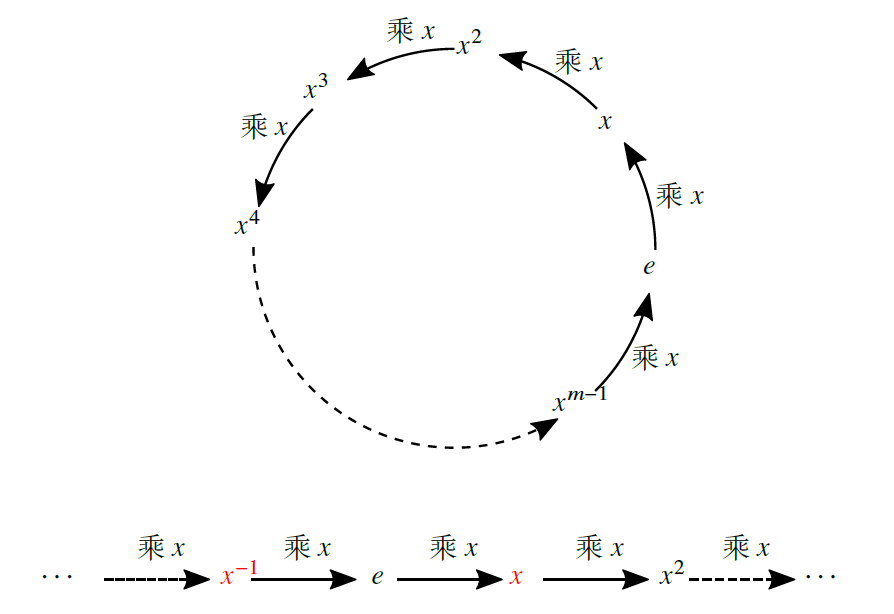
\includegraphics[scale=0.4]{有限循环群和无线循环群.png}
\label{figure:有限循环群和无线循环群}
\caption{有限循环群和无线循环群}
\end{figure}
\end{note}

\begin{proposition}\label{proposition:由x生成的群就是由子集{x}生成的子群}
设 $(G,\cdot)$ 是一个群,对$\forall x\in G$,都有 $\langle x\rangle=\langle\{x\}\rangle$.
\end{proposition}
\begin{note}
这个命题表明:由$x$生成的群就是由子集$\{x\}$生成的子群.
\end{note}
\begin{proof}
根据定义和性质,$\langle\{x\}\rangle$ 是包含了 $\{x\}$ 的最小的子群。因此要证明这个最小的子群就是 $\langle x\rangle$,我们只须证明两点。一,$\langle x\rangle$ 是个子群;二,如果一个子群 $H$ 包含了 $\{x\}$,那么它一定要包含整个 $\langle x\rangle$。

首先,由\hyperref[proposition:<x>是一个子群]{命题\ref{proposition:<x>是一个子群}}可知$\langle x\rangle$ 是个子群。这就证明了第一点。

第二点几乎也是显然的。我们设 $H$ 是个子群,且 $x\in H$。那么根据子群包含单位元,且有乘法和逆元的封闭性,我们有 $e\in H$,并且递归地,对于 $\forall n\in\mathbb{N}_1$,都有$x^n = x\cdots x\in H$,$x^{-n}=x^{-1}\cdots x^{-1}\in H$。这就证明了 $H\supset\langle x\rangle$。 
\end{proof}

\begin{proposition}\label{proposition:有限循环群的元素可用枚举法全部列举出来}
设 $G = \langle x\rangle$ 是有限循环群,并且 $|x| = n$,则 $G=\{e,x,x^2,\cdots,x^{n - 1}\}$,并且$\{e,x,x^2,\cdots,x^{n - 1}\}$中的这些元素是两两不同的。我们称这样的有限循环群的阶是 $n$。
\end{proposition}
\begin{proof}
我们来证明两件事。第一,每一个 $G$ 中   元素都可以写成从 $0$ 开始的前 $n$ 项幂的形式;第二,从 $0$ 开始的前 $n$ 项幂是两两不同的。

我们来证明第一点。任取 $G$ 中元素 $x^m$,其中 $m\in\mathbb{Z}$。根据带余除法,存在$q\in\mathbb{Z}$,$0\leq r\leq n - 1$,使得 $m = qn + r$.那么因为 $x^n = e$,所以 $x^m = x^{qn + r}=(x^n)^q\cdot x^r = x^r$,而这就属于从 $0$ 开始的前 $n$ 项幂。

我们来证明第二点。用反证法,假设 $0\leq m' < m\leq n - 1$,使得 $x^m = x^{m'}$,则 $x^{m - m'} = e$。其中 $1\leq m - m'\leq n - 1 < n$,可是 $n = |x|$ 是最小的正整数 $k$ 使 $x^k = e$,这就导致了矛盾。

综上所述,$G=\{e,x,x^2,\cdots,x^{n - 1}\}$,其中枚举法中的这些元素是两两不同的。 
\end{proof}

\begin{proposition}
对于任意的 $n\in\mathbb{N}_1$,所有 $n$ 阶的循环群都是互相同构的.
\end{proposition}
\begin{proof}
设 $G = \langle x\rangle, G' = \langle y\rangle$ 都是 $n$ 阶循环群。令
\begin{align*}
f:G\rightarrow G'
,
x^m\mapsto y^m
\end{align*}
则对$\forall x^{m_1},x^{m_2}\in G$,其中$1\leq m_1,m_2\leq n-1$.我们都有
\begin{align*}
f\left( x^{m_1}x^{m_2} \right) =f\left( x^{m_1+m_2} \right) =y^{m_1+m_2}=y^{m_1}y^{m_2}=f\left( x^{m_1} \right) f\left( x^{m_2} \right) .
\end{align*}
因此$f$是个同态映射.
此外,它是个双射,因为我们可以明确地找到其逆映射
\begin{align*}
f^{-1}(y^m)&=x^m
\end{align*}
这样,$f$ 既是双射,也是同态,这就证明了 $f$ 是个同构。 
\end{proof}

\begin{proposition}\label{proposition:每一个无限循环群都对应两个生成元}
令 $G = \langle x\rangle$ 是无限循环群,则 $x^n(n\in\mathbb{Z})$ 是两两不同的,且 $G$ 只有两个生成元,分别是 $x$ 与 $x^{-1}$。
\end{proposition}
\begin{note}
显然,$(\mathbb{Z},+)$就是一个无限循环群,生成元是1或-1.
\end{note}
\begin{proof}
首先证明 $x^n(n\in\mathbb{Z})$ 是两两不同的。假设有两个相同,不失一般性假设 $m > n\in\mathbb{Z},x^m = x^n$,则 $x^{m - n}=e$,故 $x$ 是有有限阶的。这就矛盾了。

接着,如果 $x^n(n\in\mathbb{Z})$ 可以生成这个群,那么 $x\in\langle x^n\rangle$,于是存在 $m\in\mathbb{Z}$ 使得 $x=(x^n)^m$,于是 $x^{nm - 1}=e$。由于 $x$ 是无限阶的,所以 $nm = 1$,那么这样的 $n$ 只能是 $\pm1$。另外,显然 $x^{-1}$ 也可以生成这个群。这就证明了恰好是这两个生成元。
\end{proof}

\begin{proposition}\label{proposition:所有的无限循环群是彼此同构的}
所有的无限循环群是彼此同构的。 
\end{proposition}
\begin{note}
这个命题告诉我们:要研究无限循环群,只要研究整数加群$(\mathbb{Z},+)$就可以了.
\end{note}
\begin{proof}
设 $G = \langle x\rangle, G' = \langle y\rangle$ 都是 无限循环群。令
\begin{align*}
f:G\rightarrow G'
,
x^m\mapsto y^m
\end{align*}
则对$\forall x^{m_1},x^{m_2}\in G$,其中$m_1,m_2\in \mathbb{Z}$.我们都有
\begin{align*}
f\left( x^{m_1}x^{m_2} \right) =f\left( x^{m_1+m_2} \right) =y^{m_1+m_2}=y^{m_1}y^{m_2}=f\left( x^{m_1} \right) f\left( x^{m_2} \right) .
\end{align*}
因此$f$是个同态映射.
此外,它是个双射,因为我们可以明确地找到其逆映射
\begin{align*}
f^{-1}(y^m)&=x^m
\end{align*}
这样,$f$ 既是双射,也是同态,这就证明了 $f$ 是个同构。
\end{proof}

\begin{proposition}\label{proposition:有限循环群的阶的计算公式}
令 $G = \langle x\rangle$ 是一个 $n$ 阶循环群。假设 $1\leq m\leq n$,则 $x^m$ 的阶为
\begin{align*}
|x^m|=\frac{n}{\gcd(n,m)}.
\end{align*}
\end{proposition}
\begin{proof}
设 $1\leq m\leq n - 1$,我们希望找到最小的正整数 $k$ 使得 $(x^m)^k = x^{mk}=e$。由于 $|x| = n$,故这等价于 $n\mid mk$。接下来我们要利用简单的初等数论。通过同时除以 $n$ 和 $m$ 的最大公因数,我们得到
\begin{align*}
\frac{n}{\gcd(n,m)}\Bigg|\frac{m}{\gcd(n,m)}\cdot k
\end{align*}
而因为 $\frac{n}{\gcd(n,m)}$ 和 $\frac{m}{\gcd(n,m)}$ 是互素的,所以这个条件进一步等价于
\begin{align*}
\frac{n}{\gcd(n,m)}\Bigg|k
\end{align*}
也就是说,最小的这个正整数 $k$ 正是 $\frac{n}{\gcd(n,m)}$。这就完成了证明.
\end{proof}

\begin{proposition}
令 $G = \langle x\rangle$ 是一个 $n$ 阶循环群,则 $x^m(1\leq m\leq n)$ 是个生成元,当且仅当
\begin{align*}
\gcd(m,n)=1.
\end{align*}
根据欧拉 $\phi$ 函数的定义,这些生成元的个数正是 $\phi(n)$。 
\end{proposition}
\begin{proof}
若$x^m$是一个生成元,则由$G$是一个$n$阶循环群可知,$|x^m|=n$.从而由\hyperref[proposition:有限循环群的阶的计算公式]{命题\ref{proposition:有限循环群的阶的计算公式}}可知,$\gcd(m,n)=\frac{n}{|x^m|}=1$.

若$\gcd(m,n)=1$,则由\hyperref[proposition:有限循环群的阶的计算公式]{命题\ref{proposition:有限循环群的阶的计算公式}}可知,$|x^m|=\frac{n}{\gcd(n,m)}=n$.从而
\begin{align*}
\left( x^m \right) ^n=e,\,\left( x^m \right) ^{n+1}=\left( x^m \right) ^nx=x,\cdots ,\left( x^m \right) ^{2n-1}=\left( x^m \right) ^nx^{n-1}=x^{n-1}.
\end{align*}
又由\hyperref[proposition:有限循环群的元素可用枚举法全部列举出来]{命题\ref{proposition:有限循环群的元素可用枚举法全部列举出来}}可知$G=\{e,x,\cdots,x^{n-1}\}$.于是
\begin{align*}
G=\left\{ e,x,\cdots ,x^{n-1} \right\} =\left\{ \left( x^m \right) ^n,\left( x^m \right) ^{n+1},\cdots ,\left( x^m \right) ^{2n-1} \right\}=\left\{ \left( x^m \right) ^n:n\in \mathbb{Z} \right\} .
\end{align*}
因此$G=\langle x^m\rangle$,故$x^m$是$G$的生成元.
\end{proof}

\begin{definition}[群的阶]
设$(G,\cdot)$是一个群,则$G$的阶,记作$|G|$,定义为$G$的集合大小(元素的个数).
\end{definition}

\begin{definition}[子群的阶]
设$(G,\cdot)$是一个群,$H$是$G$的子群,则$H$的阶,记作$|H|$,定义为$H$的集合大小(元素的个数)。若$H$是无限群则记$|H| = \infty$。
\end{definition}

\begin{definition}[左陪集]
设$G$是一个群,$H < G$是一个子群,$a \in G$。则称$aH$是$H$的一个(由$a$引出的)\textbf{左陪集},定义为
\begin{align*}
aH = \{ax : x \in H\}.
\end{align*} 
\end{definition}
\begin{remark}
$aH$一般来说不是$G$的子群.
\end{remark}

\begin{lemma}
令$G$是一个有限群,$H < G$是一个子群,$a \in G$。令
\begin{align*}
f : H \to aH,x \mapsto ax.
\end{align*}
则$f$是一个双射。特别地,$|H| = |aH|$。 
\end{lemma}
\begin{proof}

\end{proof}

\begin{proposition}
令$G$是一个有限群,$H < G$是一个子群,$a,b \in G$。则左陪集$aH$和$bH$要么相等,要么无交。也就是说,我们有$aH = bH$,或$aH \cap bH = \emptyset$。
\end{proposition}
\begin{proof}
假设$a,b \in G$。不妨假设$aH\cap bH \neq \emptyset$,假设$ah_1 = bh_2 \in aH\cap bH$,其中$h_1,h_2 \in H$。我们只须证明$aH = bH$,而根据对称性,我们只须证明$aH \subset bH$即可。任取$aH$中的元素$ah (h \in H)$,则
\begin{align*}
ah=(bh_2h_1^{-1})h = b(h_2h_1^{-1}h) \in bH
\end{align*}
这就完成了证明.
\end{proof}

\begin{theorem}

\end{theorem}

\begin{definition}

\end{definition}

\begin{proposition}

\end{proposition}
\begin{proof}

\end{proof}

\begin{theorem}

\end{theorem}
\begin{proof}

\end{proof}

\begin{definition}

\end{definition}

\begin{proposition}

\end{proposition}
\begin{proof}

\end{proof}

\begin{theorem}

\end{theorem}
\begin{proof}

\end{proof}

\begin{definition}

\end{definition}

\begin{proposition}

\end{proposition}
\begin{proof}

\end{proof}

\begin{theorem}

\end{theorem}
\begin{proof}

\end{proof}

\begin{definition}

\end{definition}

\begin{proposition}

\end{proposition}
\begin{proof}

\end{proof}

\begin{theorem}

\end{theorem}
\begin{proof}

\end{proof}


\end{document}